\documentclass[utf8]{beamer}
\usepackage{cmap}
\usepackage [utf8]{inputenc}
\usepackage[russian]{babel}
\usepackage[backend=bibtex]{biblatex}
\bibliography{DipBib}
\usepackage[T2A]{fontenc}
\usepackage{cmap}
\newsavebox{\longestsec}
\usetheme{Madrid}
\useoutertheme{tree}
\usepackage{epstopdf}
\DeclareGraphicsExtensions{.eps} 

\newtheorem{mdefinition}{Определение}[section]
\newtheorem{mremark}{Примечание}[subsection]
\newtheorem{msuggest}{Предложение}[subsection]
\newtheorem{mclaim}{Утверждение}[subsection]
\newtheorem{mlemma}{Лемма}[subsection]
\newtheorem{mtheorem}{Теорема}
\newtheorem{mconseq}{Следствие}

\DeclareMathOperator{\argmax}{argmax}
\DeclareMathOperator{\argmin}{argmin}
\DeclareMathOperator{\grad}{grad}
\DeclareMathOperator{\sign}{sign}
\DeclareMathOperator{\diag}{diag}
\DeclareMathOperator{\norm}{norm}

\title{Сходимость численных методов вероятностного тематического моделирования.}
\date{22 июня 2016}
\author{Ирхин Илья Александрович}

\institute{
 Кафедра анализа данных \\
    \vspace{0.7cm}
    Научный руководитель:  д.ф.-м.н. Воронцов Константин Вячеславович \\
    \vspace{0.7cm}
}

\begin{document}
	\begin{frame}
		\titlepage
	\end{frame}

	\begin{frame}
		\frametitle{Краткое содержание}
		\renewcommand{\baselinestretch}{1.5}
		\fontsize{12pt}{9.2}\selectfont
		\tableofcontents
	\end{frame}
	
	\section{Постановка задачи}
	\subsection{Формулировка задачи}
	
	
	\begin{frame}
		\frametitle{Тематическое моделирование текстовых коллекций}
		\textbf{Дано:}  $p(w|d) = \frac{n_{wd}}{n_d}$ -- частоты слов $w$ в документах $d$.\\
		\textbf{Найти:} $p(w|t)$ и $p(t|d)$ т.ч.
		\[
		 	p(w|d) = \sum_t p(w|t) p(t|d).
		\]
		\textbf{Критерий поиска:}  максимизация логарифма правдоподобия
		\[
\sum_{d, w} n_{dw} \log \sum_{t} \phi_{wt} \theta_{td} \to \max
\]
	\end{frame}

	\subsection{Подход ARTM}

		\begin{frame}
		\frametitle{Подход ARTM (Additive Regularization for Topic Modeling)}
		Задача максимизации $\log$ правдоподобия \textcolor{red}{с регуляризатором $R$}\footfullcite{artmdef2}:
\[
\sum_{d, w} n_{dw} \log \sum_{t} \phi_{wt} \theta_{td}  + \textcolor{red}{R(\Phi, \Theta)}\to \max_{\Phi, \Theta},
\]

		Применив теорему Каруша-Куна-Такера, получим систему уравнений на переменные $\phi$ и $\theta$. Решение данной системы методом простых итераций даст ЕМ алгоритм.

\end{frame}


 
		\begin{frame}
		\frametitle{Подход ARTM (Additive Regularization for Topic Modeling)}   
   \textbf{E-step:}
    
    \ \ \ \ $p_{tdw} = p(t|d, w) = \norm_t(\varphi_{wt} \theta_{td})$

    \medskip\textbf{M-step:}
    
    \ \ \ \ $n_{wt} = \sum\limits_{d} n_{dw} p_{tdw}$,\ \ \ $r_{wt} =  \phi_{wt}\dfrac{\partial R}{\partial\phi_{wt}}$,\ \ \  $\phi_{wt}   = \norm_w\big(n_{wt} + r_{wt}\big)$

\ \ \ \ $n_{td} = \sum\limits_{w} n_{dw} p_{tdw}$,\ \ \  \ $r_{td} =  \theta_{td}\dfrac{\partial R}{\partial\theta_{td}}$,\ \ \ \ \ $\theta_{td} = \norm_t  \big(n_{td} + r_{td}\big)$
    \ \\
    \ \\
	где $norm_y(x) = \frac{(x)_{+}}{\sum\limits_y (x)_{+}}$, и $(x)_{+} = \max(x, 0)$\footfullcite{artmdef3}.


	\end{frame}

	\section{Исследование сходимости ARTM}
	\subsection{Цели работы}
	
	\begin{frame}
		\frametitle{Цели работы}

\begin{enumerate}
\item Изучение свойств сходимости алгоритма ARTM. 
\item Поиск конструктивных условий на регуляризаторы, способствующих сходимости.
\item Анализ возможных модификаций алгоритма, улучшающих его сходимость.
\item Проведение эксперимента для проверки выполнения полученных условий, а также сравнения предложенных модификаций и стандартного алгоритма ARTM.
\end{enumerate}
	\end{frame}

	\subsection{Полученные результаты}
	
	\begin{frame}
		\frametitle{Основная теорема о сходимости}
\footnotesize{
Под $x^k$ понимается значение $x$ на $k$-ой итерации. Пусть выполнены следующие условия:
\begin{enumerate}
\item  $ n^k_{wt} = 0 \Rightarrow \phi^k_{wt} = 0$ -- сохранение нуля.
\item $n^k_{td} = 0 \Rightarrow \theta^k_{td} = 0$ -- сохранение нуля.
\item $\exists \varepsilon>0\ \exists N\ \forall k > N\ \phi^k_{wt}, \theta^k_{td} \notin (0, \varepsilon)$ -- отделимость от нуля.
\item  $ n_{dw}>0 \Rightarrow \forall k\ \exists t\colon p^k_{tdw} > 0$ -- невырожденность распределения $ p(t|d,w)$.
\item $\exists \delta\geq 0\ \exists N\ \forall k > N \ \forall t\ \exists w\  n^k_{wt} + r^k_{wt} > \delta$ -- невырожденность $p(w|t)$.
\item $\exists \delta\geq 0\ \exists N\ \forall k > N \ \forall d\ \exists t\  n^k_{td} + r^k_{td} > \delta$ -- невырожденность $p(t|d)$.
\item $\exists N\ \forall k > N\colon\ \ Q^k (\phi^k, \theta^k)+ R(\phi^k, \theta^k) \geq Q^k(\phi^{k-1}, \theta^{k-1}) + R(\phi^{k-1}, \theta^{k-1})$, где $Q^k(\phi, \theta) = \sum\limits_{t,d,w} p^k_{tdw} (\ln \phi_{wt} + \ln \theta_{td})$ --  монотонное неубывание нижней оценки правдоподобия.
\end{enumerate}
Тогда выполнено:
\[
KL(p_{tdw}^{k}||p_{tdw}^{k + 1}) \to 0 \text{ при } k \to \infty.
\]
\[
L(\phi^k, \theta^k) + R(\phi^k, \theta^k) \text{ монотонно сходится при } k \to \infty.
\]
}
	\end{frame}

	\begin{frame}
		\frametitle{Несколько следствий}
\begin{enumerate}
\item  Если в условии №5 и №6 $\delta > 0$, то $\phi^k_{wt} - \phi_{wt}^{k-1} \to 0$ и $\theta^k_{td} - \theta^{k-1}_{td} \to 0$.
\item Все предельные точки $\phi^k_{wt}$ и $\theta^k_{td}$ -- стационарные точки $L + R$ при каком-то ограничении на множество нулевых позиций $\phi_{wt}$ и $\theta_{td}$.
\item Если множество стационарных точек $L + R$ дискретно, то $\phi_{wt}^k$ и $\theta_{td}^k$ сходятся к стационарной точке $L+R$.
\item Ряд $\sum\limits_{k=1}^{\infty} (p_{tdw}^k - p_{tdw}^{k-1})^2$ сходится.
\end{enumerate}
	\end{frame}
	

	\section{Улучшения сходимости}
	\subsection{Модификации М-шага}
	
	\begin{frame}
		\frametitle{Несмещённые оценки в  М-шаге}
Для доказательства условия №7 (увеличение $Q^k+R$ на каждой итерации) предлагается заменить все вхождения $\phi_{wt}$ и $\theta_{td}$ на их несмещённые оценки $\frac{n_{wt}}{n_t}$ и $\frac{n_{td}}{n_d}$
\[
\left\{
	\begin{aligned}
		r_{wt} =  \frac{n_{wt}}{n_t} \frac{\partial{R}}{\partial{\phi_{wt}}} \bigg(\frac{n_{wt}}{n_t}, \frac{n_{td}}{n_d}\bigg),\\
		r_{td} = \frac{n_{td}}{n_d} \frac{\partial{R}}{\partial{\theta_{td}}} \bigg(\frac{n_{wt}}{n_t}, \frac{n_{td}}{n_d}\bigg).
	\end{aligned}
\right.
\]
	\end{frame}

	
	\begin{frame}
		\frametitle{Уточнение градиента изменения}
		Для улучшения сходимости предлагается использовать градиент регуляризатора в формуле М-шага.
\[
\left\{
	\begin{aligned}
		r_{wt} =  A_t \bigg[\textcolor{red} {\frac{\partial{R}}{\partial{\phi_{wt}}} - \sum\limits_u \phi_{ut} \frac{\partial{R}}{\partial{\phi_{ut}}} }\bigg] \bigg(\frac{n_{wt}}{n_t}, \frac{n_{td}}{n_d}\bigg),\\
		r_{td} =  B_d \bigg[ \textcolor{red} {\frac{\partial{R}}{\partial{\theta_{td}}} - \sum\limits_s \theta_{sd} \frac{\partial{R}}{\partial{\theta_{sd}}} }\bigg] \bigg(\frac{n_{wt}}{n_t}, \frac{n_{td}}{n_d}\bigg),
	\end{aligned}
\right.
\]
Где $A_t$ и $B_d$ -- коэффициенты, зависящие только от темы(документа). Эту добавку можно эффективно вычислить, поскольку второе слагаемое одникаковое для всех слов (тем) в рамках одной темы (документа).
	\end{frame}

\begin{frame}
		\frametitle{Обоснование формул}
В точке  $\big( \frac{n_{wt}}{n_t}, \frac{n_{td}}{n_d}\big)$ можно найти градиент $R$ по $n_{wt}$ и $n_{td}$:
\[
\frac{\partial{R}}{\partial{n_{wt}}} = \frac{1}{n_t} \bigg(\frac{\partial{R}}{\partial{\phi_{wt}}} - \sum\limits_u \phi_{ut} \frac{\partial{R}}{\partial{\phi_{ut}}}\bigg)
\]
\[
\frac{\partial{R}}{\partial{n_{td}}} = \frac{1}{n_d} \bigg( \frac{\partial{R}}{\partial{\theta_{td}}} - \sum\limits_s \theta_{sd} \frac{\partial{R}}{\partial{\theta_{sd}}} \bigg)
\]
Для стандартной формулы преобразования можно показать, что угол с данным градиентом всегда острый, что гарантирует увеличение $R$. Тем не менее, очевидно, что наибольшее локальное увеличение будет давать именно изменение вдоль градиента.
	\end{frame}

\begin{frame}
		\frametitle{Более подробно про острый угол градиента}

Для упрощения будет рассмотрен случай $R(\Phi, \Theta) = R(\Phi)$.
\[
\frac{\partial{R}}{\partial{n_{wt}}}  = \frac{1}{n_t} \sum_{u} \bigg(\frac{\partial{R}}{\partial{\phi_{wt}}}  -  \frac{\partial{R}}{\partial{\phi_{ut}}} \bigg)  \phi_{ut}
\]
С другой стороны изменение $n_{wt}$ на итерации равно $ \Delta n_{wt} =  \phi_{wt} \frac{\partial{R}}{\partial{\phi_{wt}}}$.
\[
(\overline{\Delta n_{wt}}, grad\ R(n_{wt}, n_{td})) = \sum\limits_{w, t, u}  \frac{1}{n_{t}}  \bigg(  \frac{\partial{R}}{\partial{\phi_{wt}}}  -  \frac{\partial{R}}{\partial{\phi_{ut}}}  \bigg)  \frac{\partial{R}}{\partial{\phi_{wt}}} \phi_{wt} \phi_{ut}  = 
\]
\[
= \frac12  \sum\limits_{t, w, u}  \frac{1}{n_{t}} \bigg(  \frac{\partial{R}}{\partial{\phi_{wt}}}  -  \frac{\partial{R}}{\partial{\phi_{ut}}}  \bigg)^2 \phi_{wt} \phi_{ut}  \geq 0
\]
	\end{frame}

\begin{frame}
		\frametitle{Отличия модификаций}
Пусть $R = -\tau \sum_{w, t} \phi_{wt}$. Он не должен влиять на оптимизацию, поскольку просто равен константе при ограничениях задачи. Тем не менее, исходные формулы дадут следующий М-шаг:
\[
\left\{
	\begin{aligned}
		\phi_{wt} = \norm_w \big( n_{wt} - \tau \phi_{wt}\big),\\
		\theta_{td} = \norm_t \big( n_{td} - \tau \theta_{td}\big).
	\end{aligned}
\right.
\]
Что отличается от итерационного процесса для  PLSA. По формуле градиентной модификации получится, что 
\[
\frac{\partial{R}}{\partial{\phi_{wt}}} - \sum\limits_u \phi_{ut} \frac{\partial{R}}{\partial{\phi_{ut}}} = \tau - \tau =0
\]
То есть в точности PLSA.
	\end{frame}

	\subsection{Экспериментальные результаты}
	
	\begin{frame}
		\frametitle{Эксперимент}
		
\begin{enumerate}
\item В качестве регуляризатора был взят регуляризатор декоррелирования ($R = -\tau\sum\limits_w \sum\limits_{t \neq s} \phi_{wt} \phi_{ws}$).
\item Были проверены четыре случая величины $\tau$: $10^5,~10^6,~10^7,~10^8$, для разного числа тем: 3, 10, 30.
\item Использовались статьи со спортивного сайта sports.ru по 7 видам спорта.
\item Проверялись стандартная формула, замена несмещёнными оценками и градиентное преобразование.
\item Алгоритм  запускался из случайных начальных приближений, одинаковых для всех запусков, после чего сравнивались средние значения целевых метрик.
\end{enumerate}

	\end{frame}

	\begin{frame}
\begin{figure}
	\centering   
	\caption{Значения $L + R$. $|T| = 10$. Градиентные поправки немного хуже остальных, но при большом $\tau$ показывают ощутимо лучший результат.} 
	\medskip
	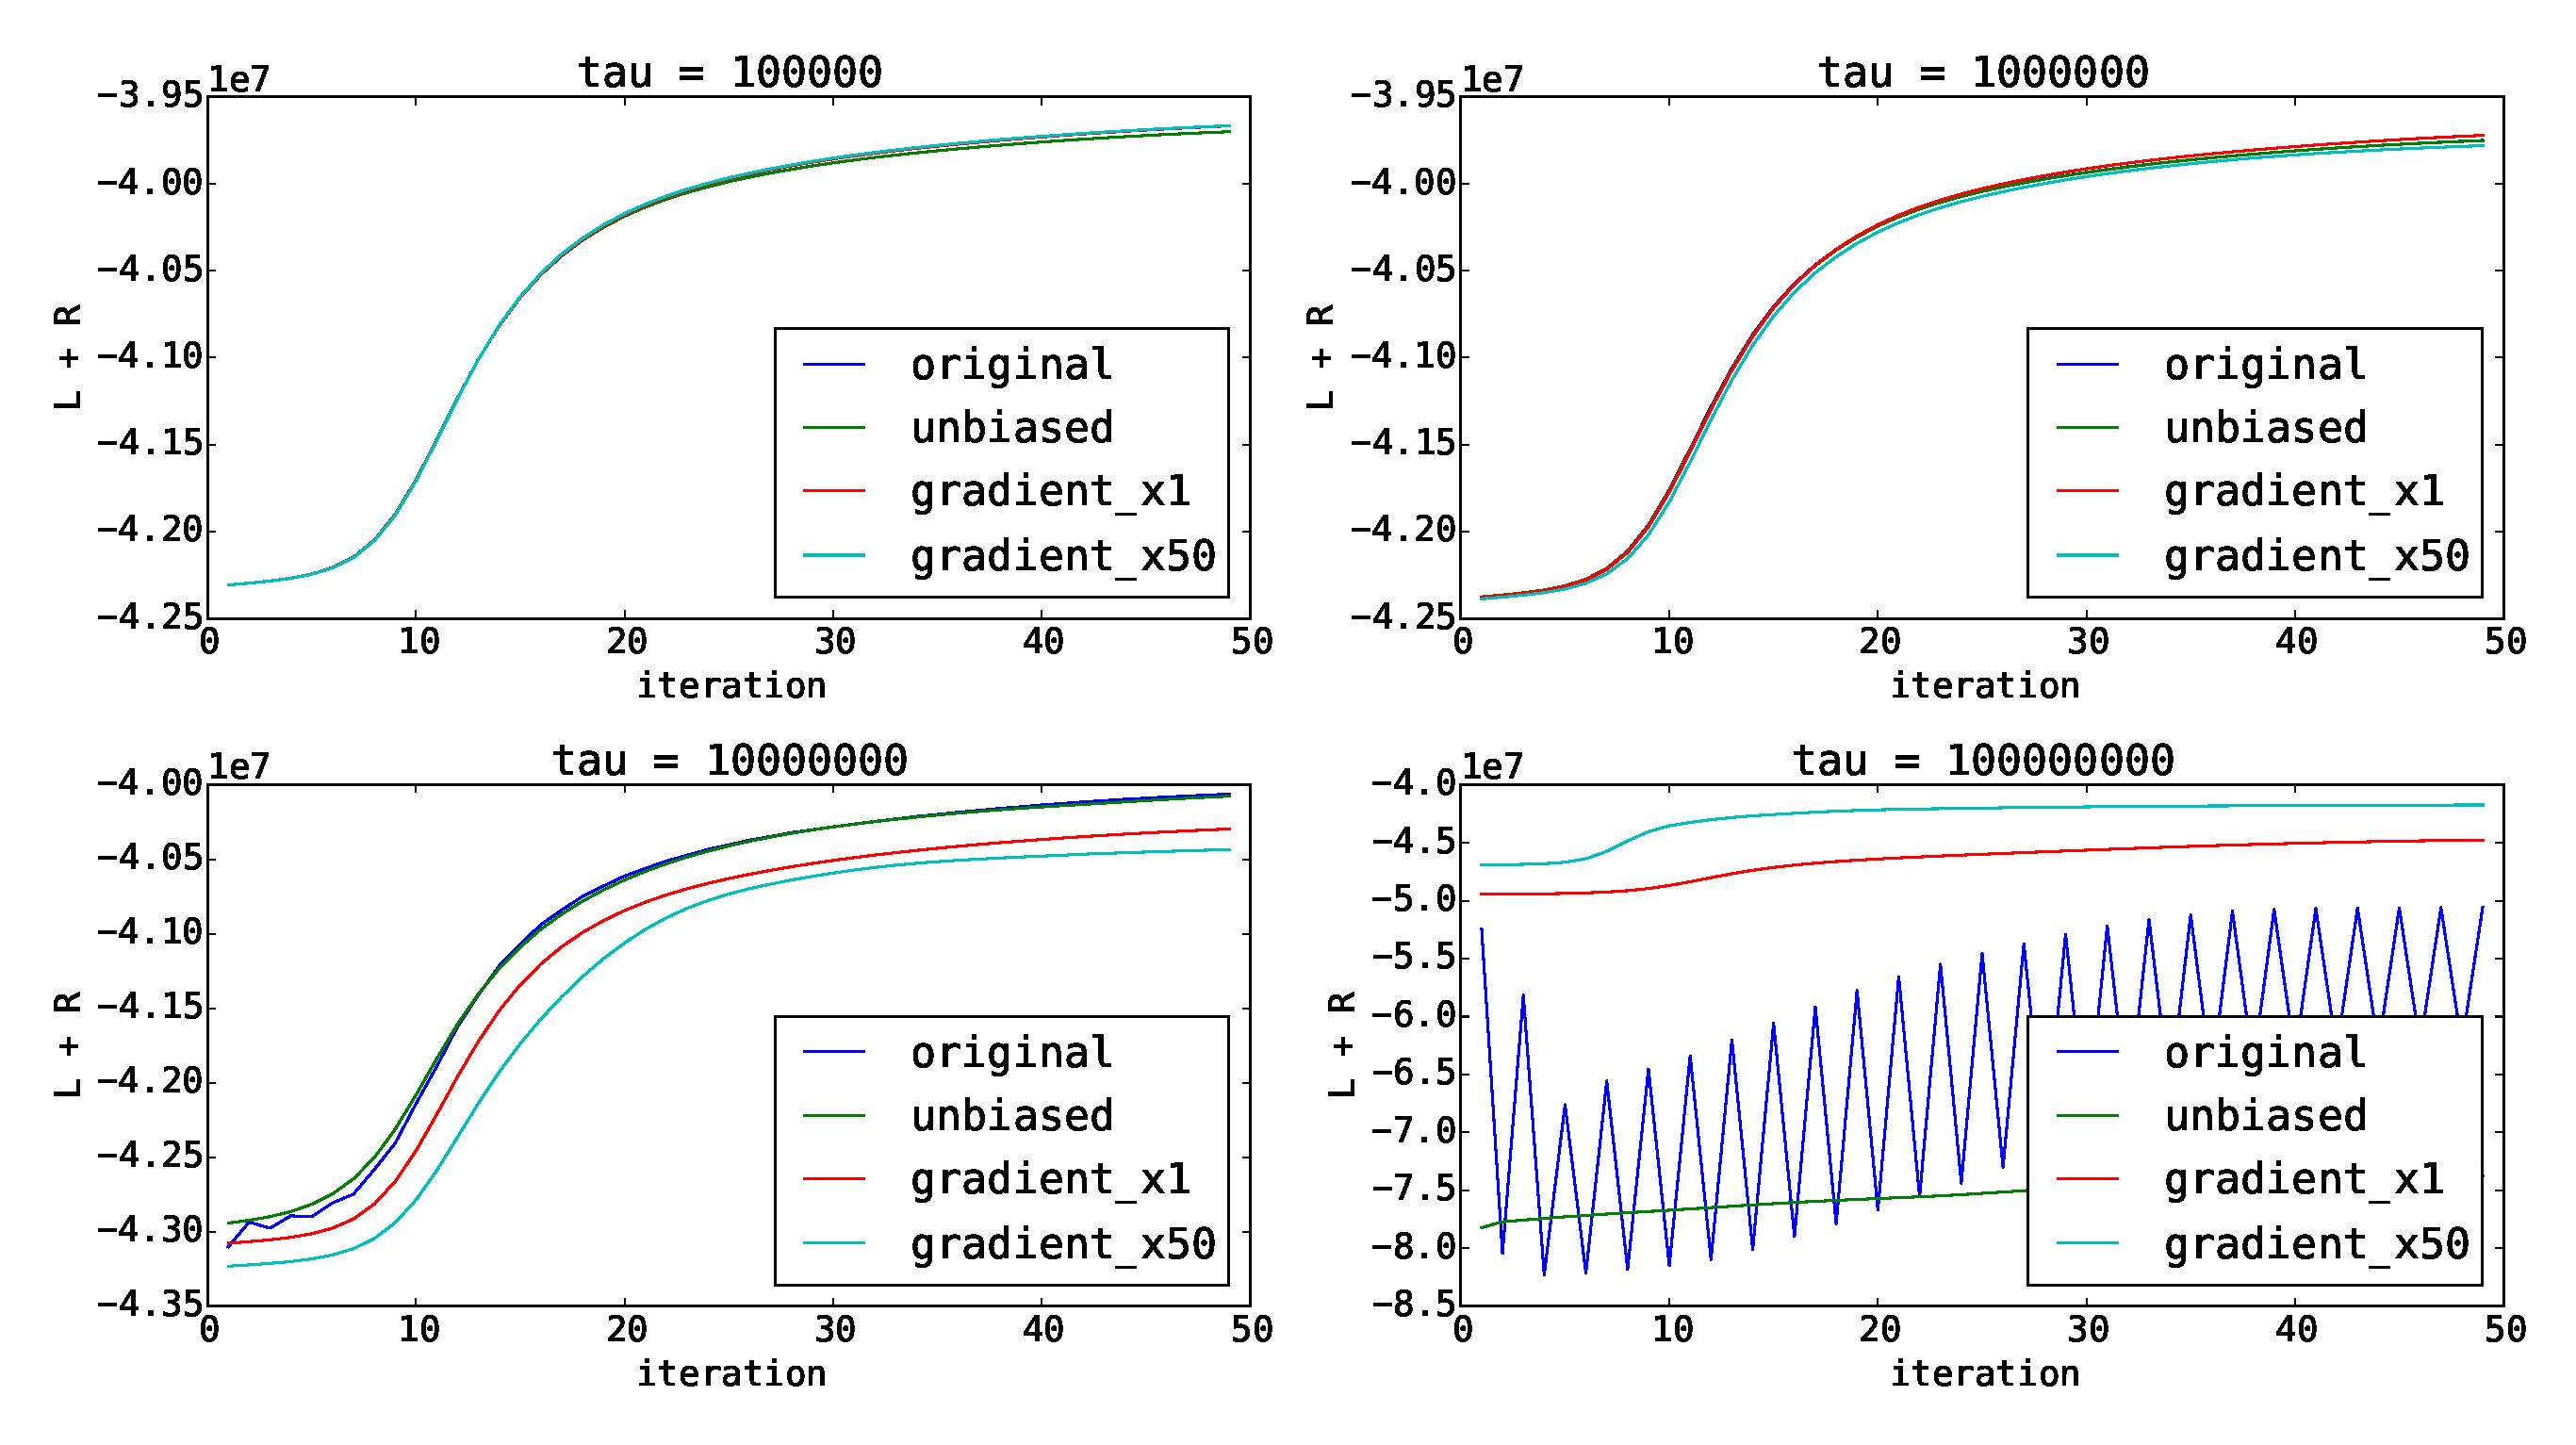
\includegraphics[width=0.9\linewidth]{presentation_pictures/topics_10_LR_values.eps}  
\end{figure}
	\end{frame}

	\begin{frame}
\begin{figure}
	\centering   
	\caption{Значения $R$. $|T| = 10$.  На верхних графиках виден скачок $R$ на первой итераций, на нижних графиках он ярче выражен. Несмещённая модификация и градиент $\times 50$  лучше всех остальных.} 
	\medskip
	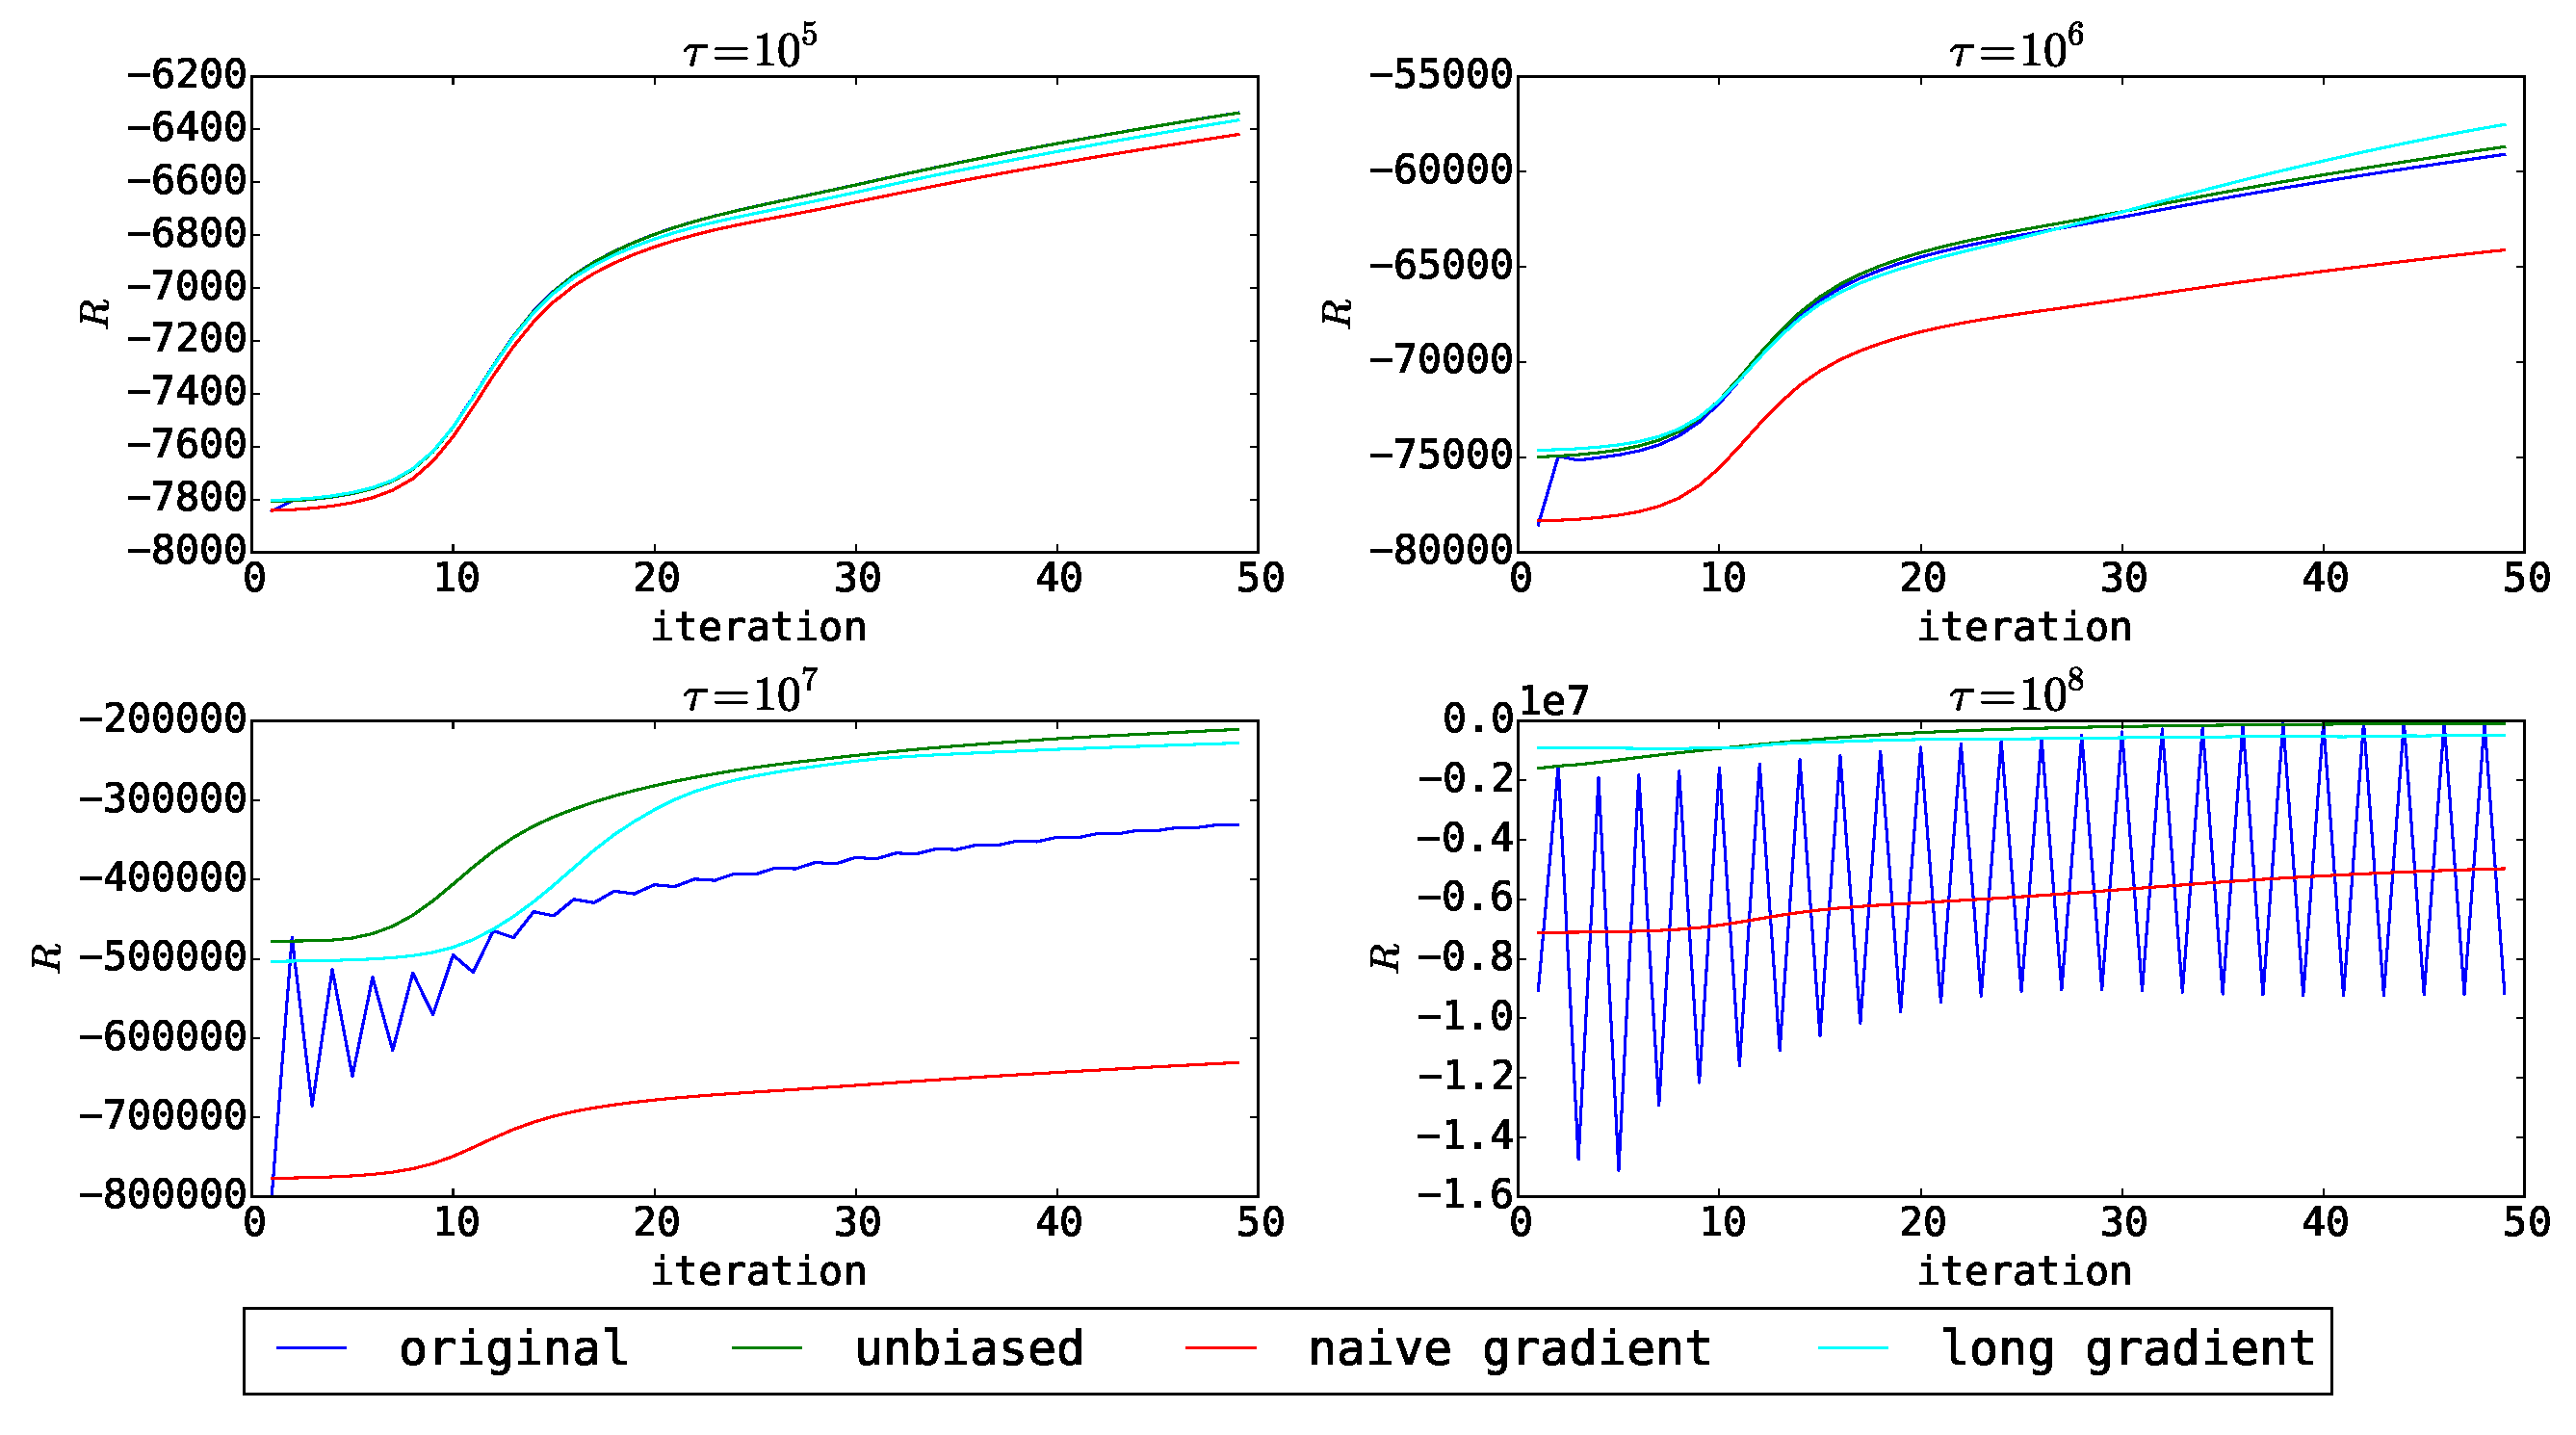
\includegraphics[width=0.9\linewidth]{presentation_pictures/topics_10_R_values.eps}  
\end{figure}
	\end{frame}
	
	\begin{frame}
\begin{figure}
	\centering   
	\caption{Значения $R$. $|T| = 30$. Эффект скачков уже ярко выражен при $\tau = 10^6$. Градиент $\times 50$ существенно лучше всех остальных.} 
	\medskip
	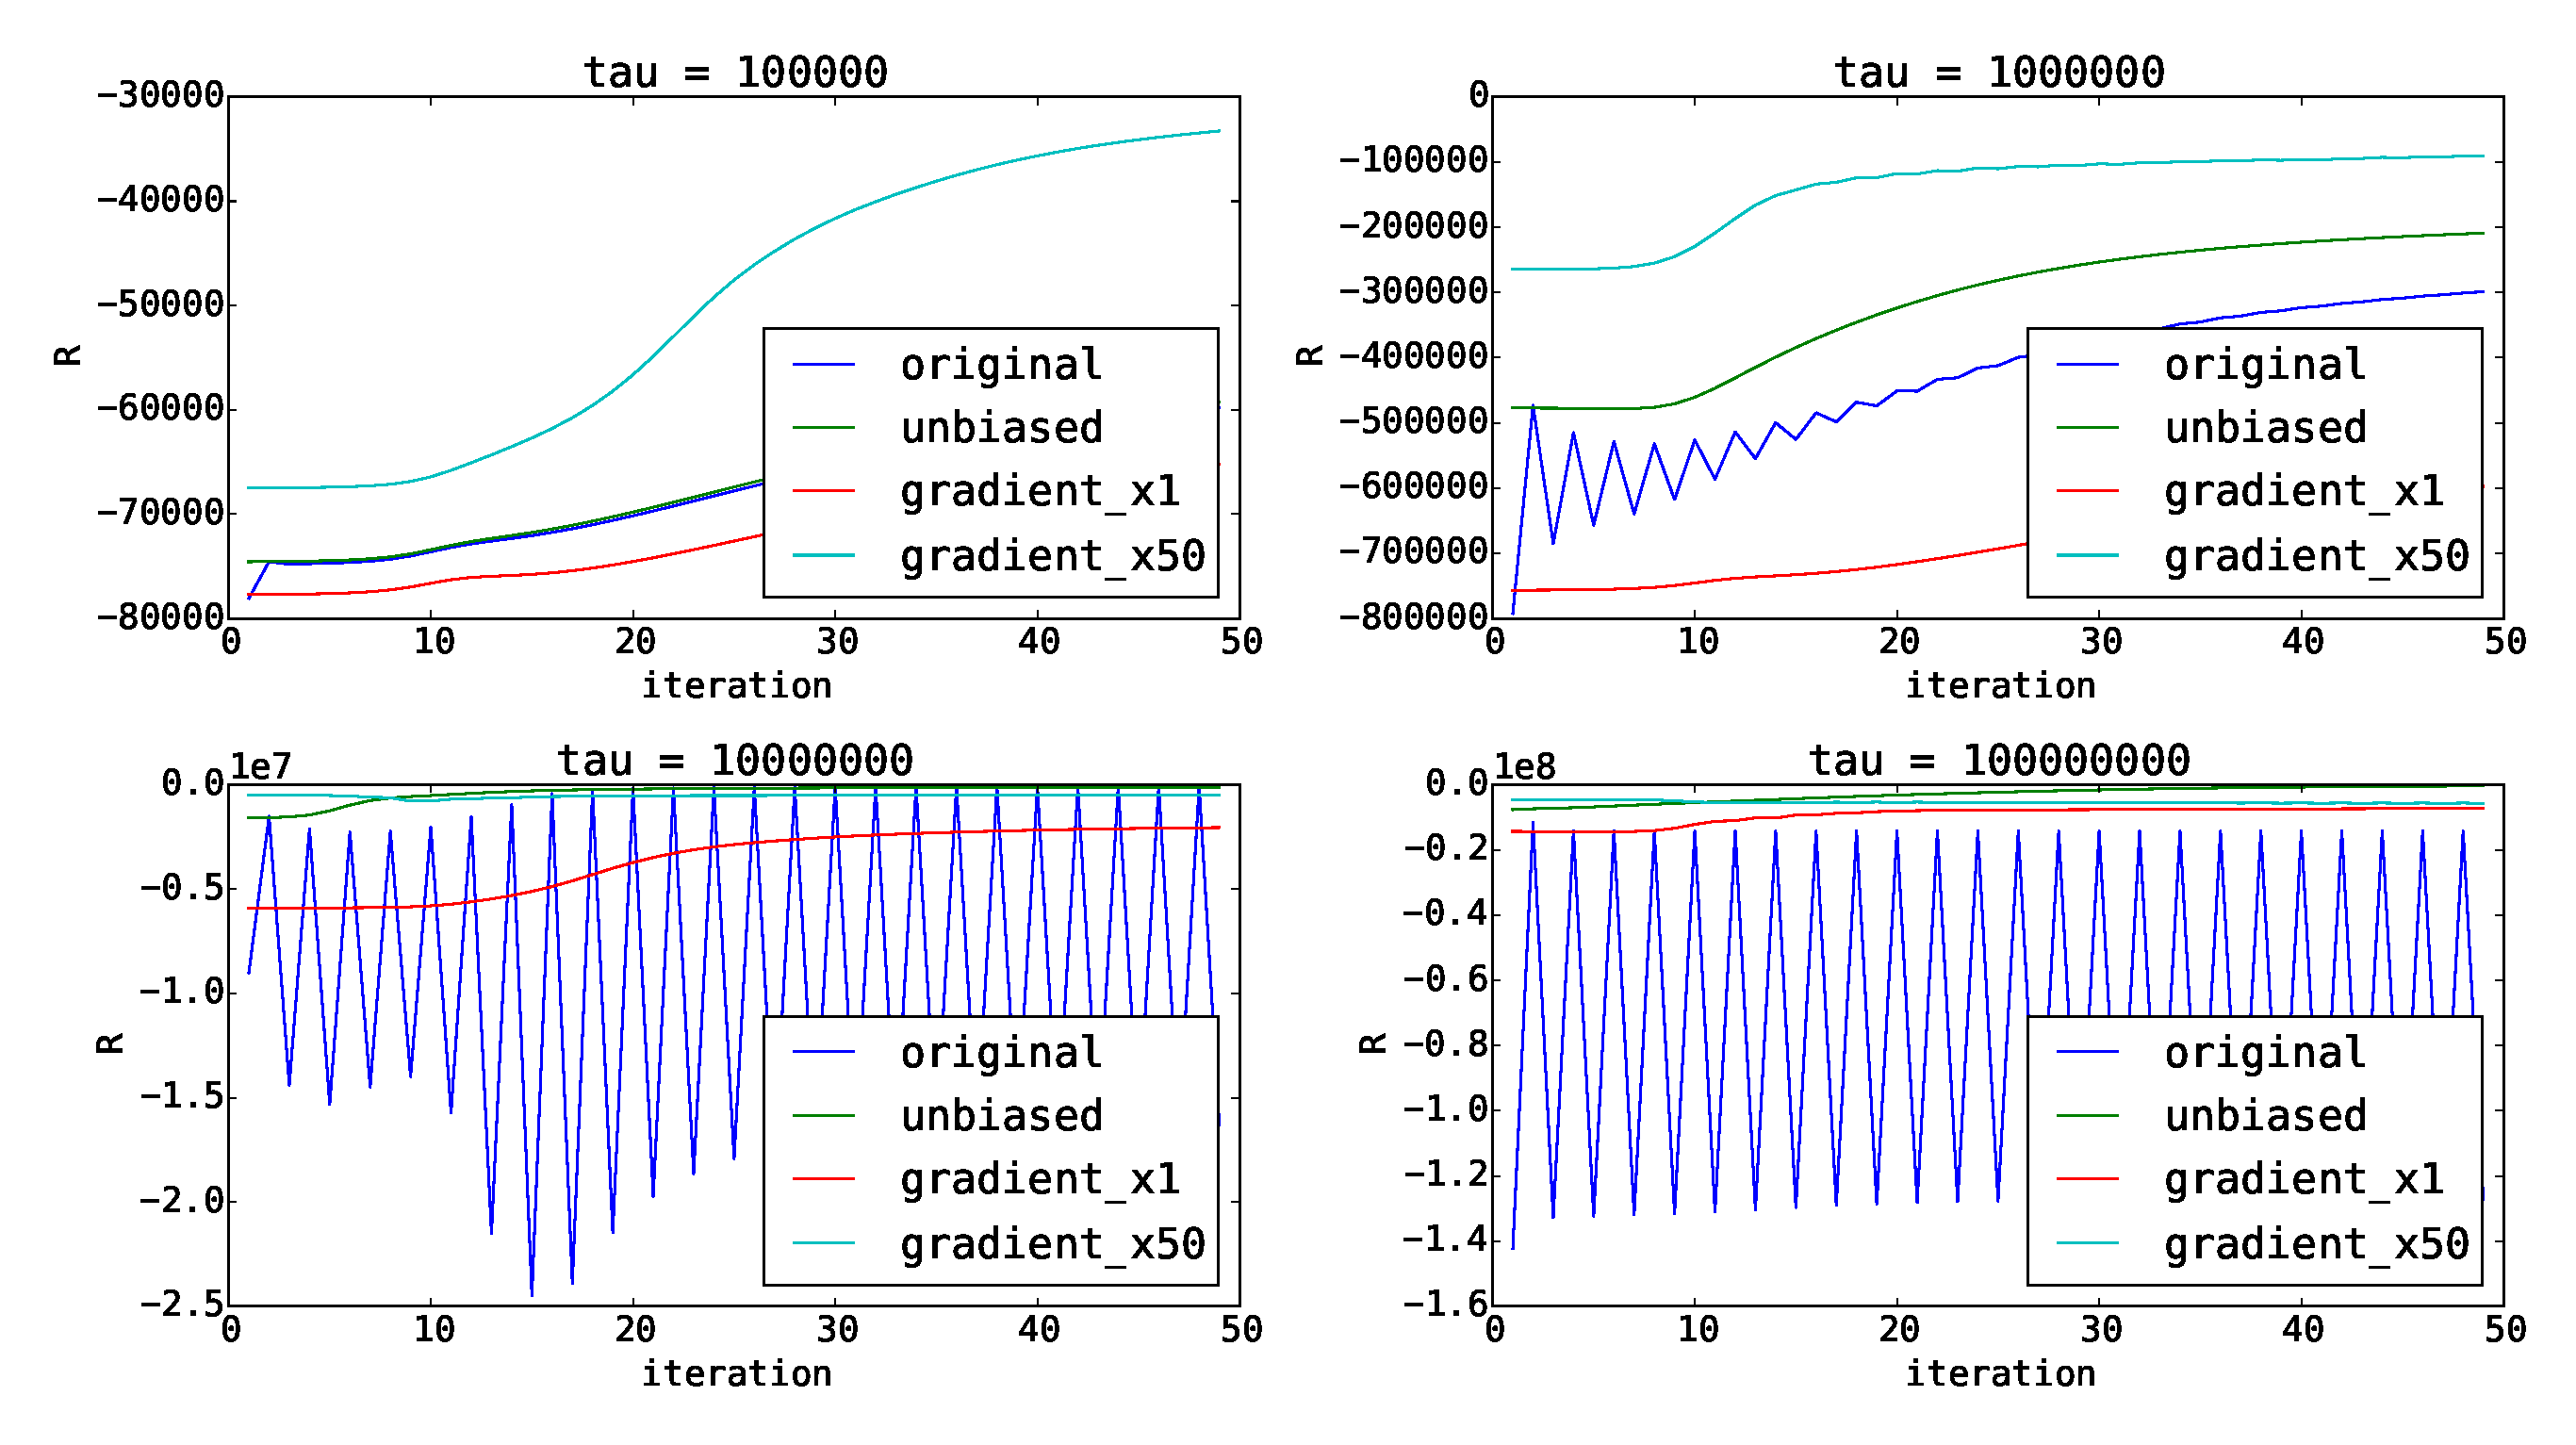
\includegraphics[width=0.9\linewidth]{presentation_pictures/topics_30_R_values.eps}  
\end{figure}
	\end{frame}
	
	\begin{frame}
\begin{figure}
	\centering
	\caption{Изменение $R$ на M-шаге. $|T| = 10$.}    
	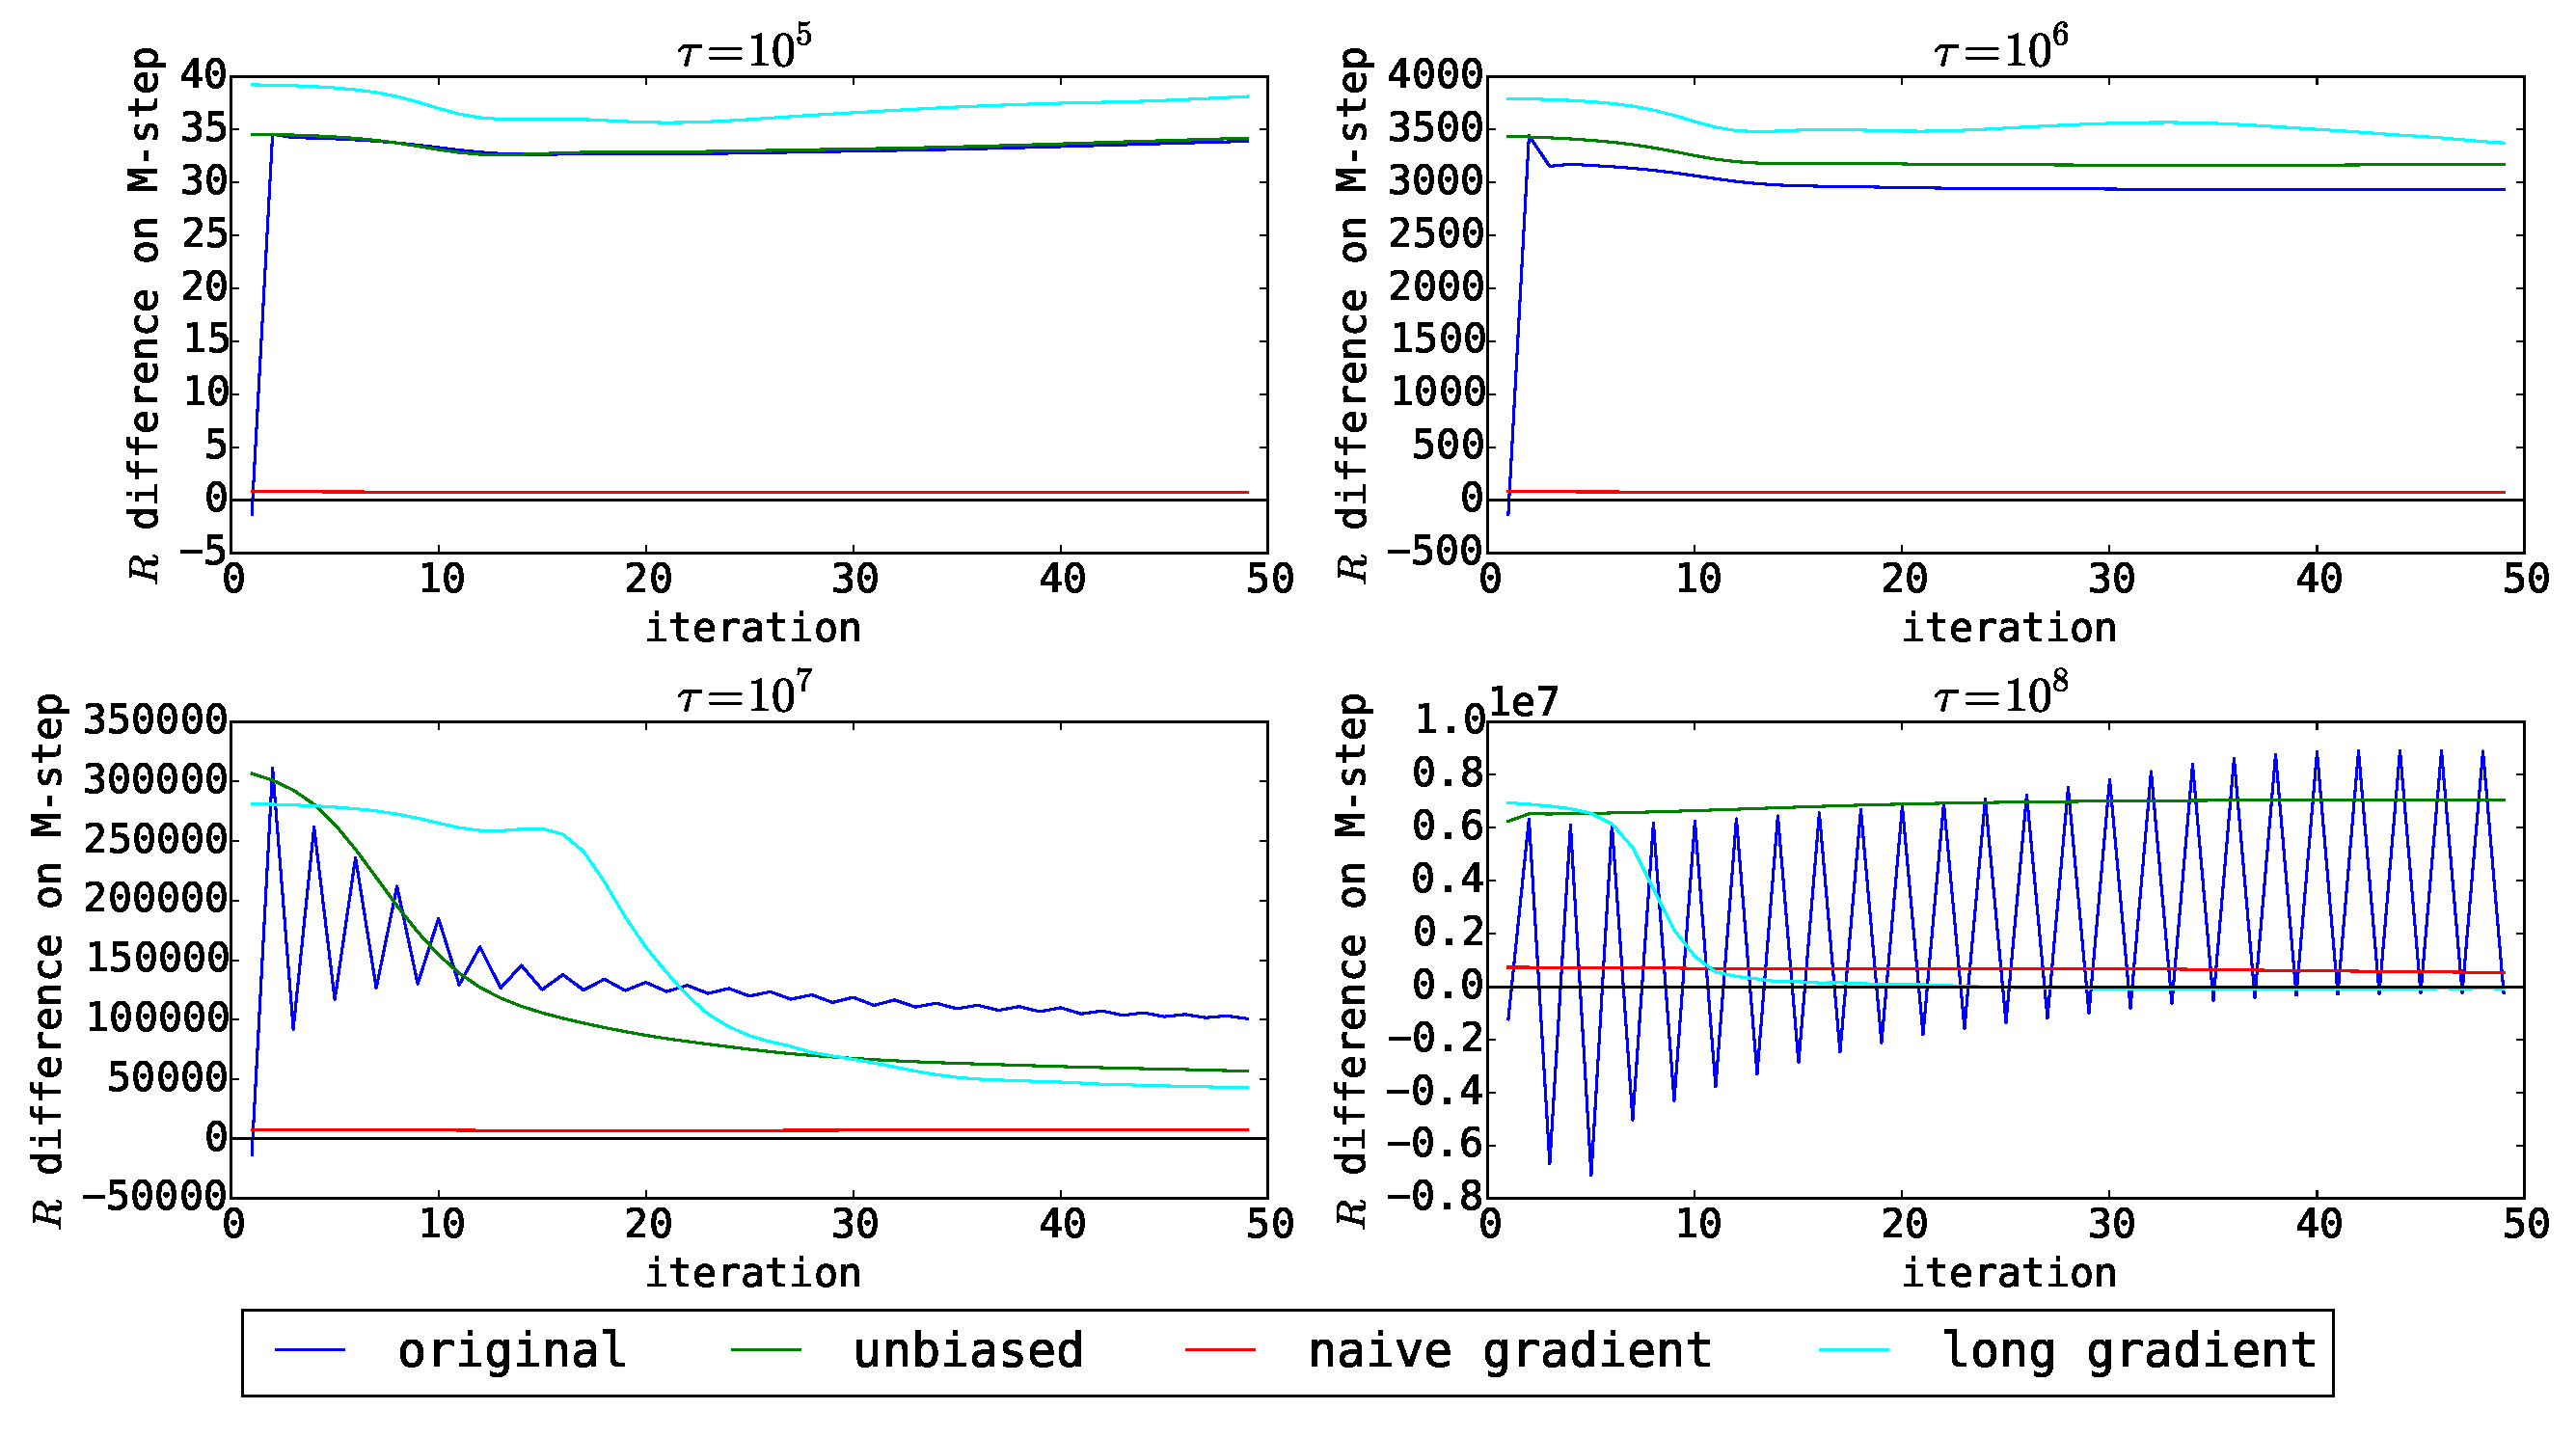
\includegraphics[width=1.0\linewidth]{presentation_pictures/topics_10_RMstepDiff}
\end{figure}
	\end{frame}
	
	\begin{frame}
\begin{figure}
	\centering
	\caption{Удельное изменение $R$ на M-шаге. $|T| = 10$.}    
	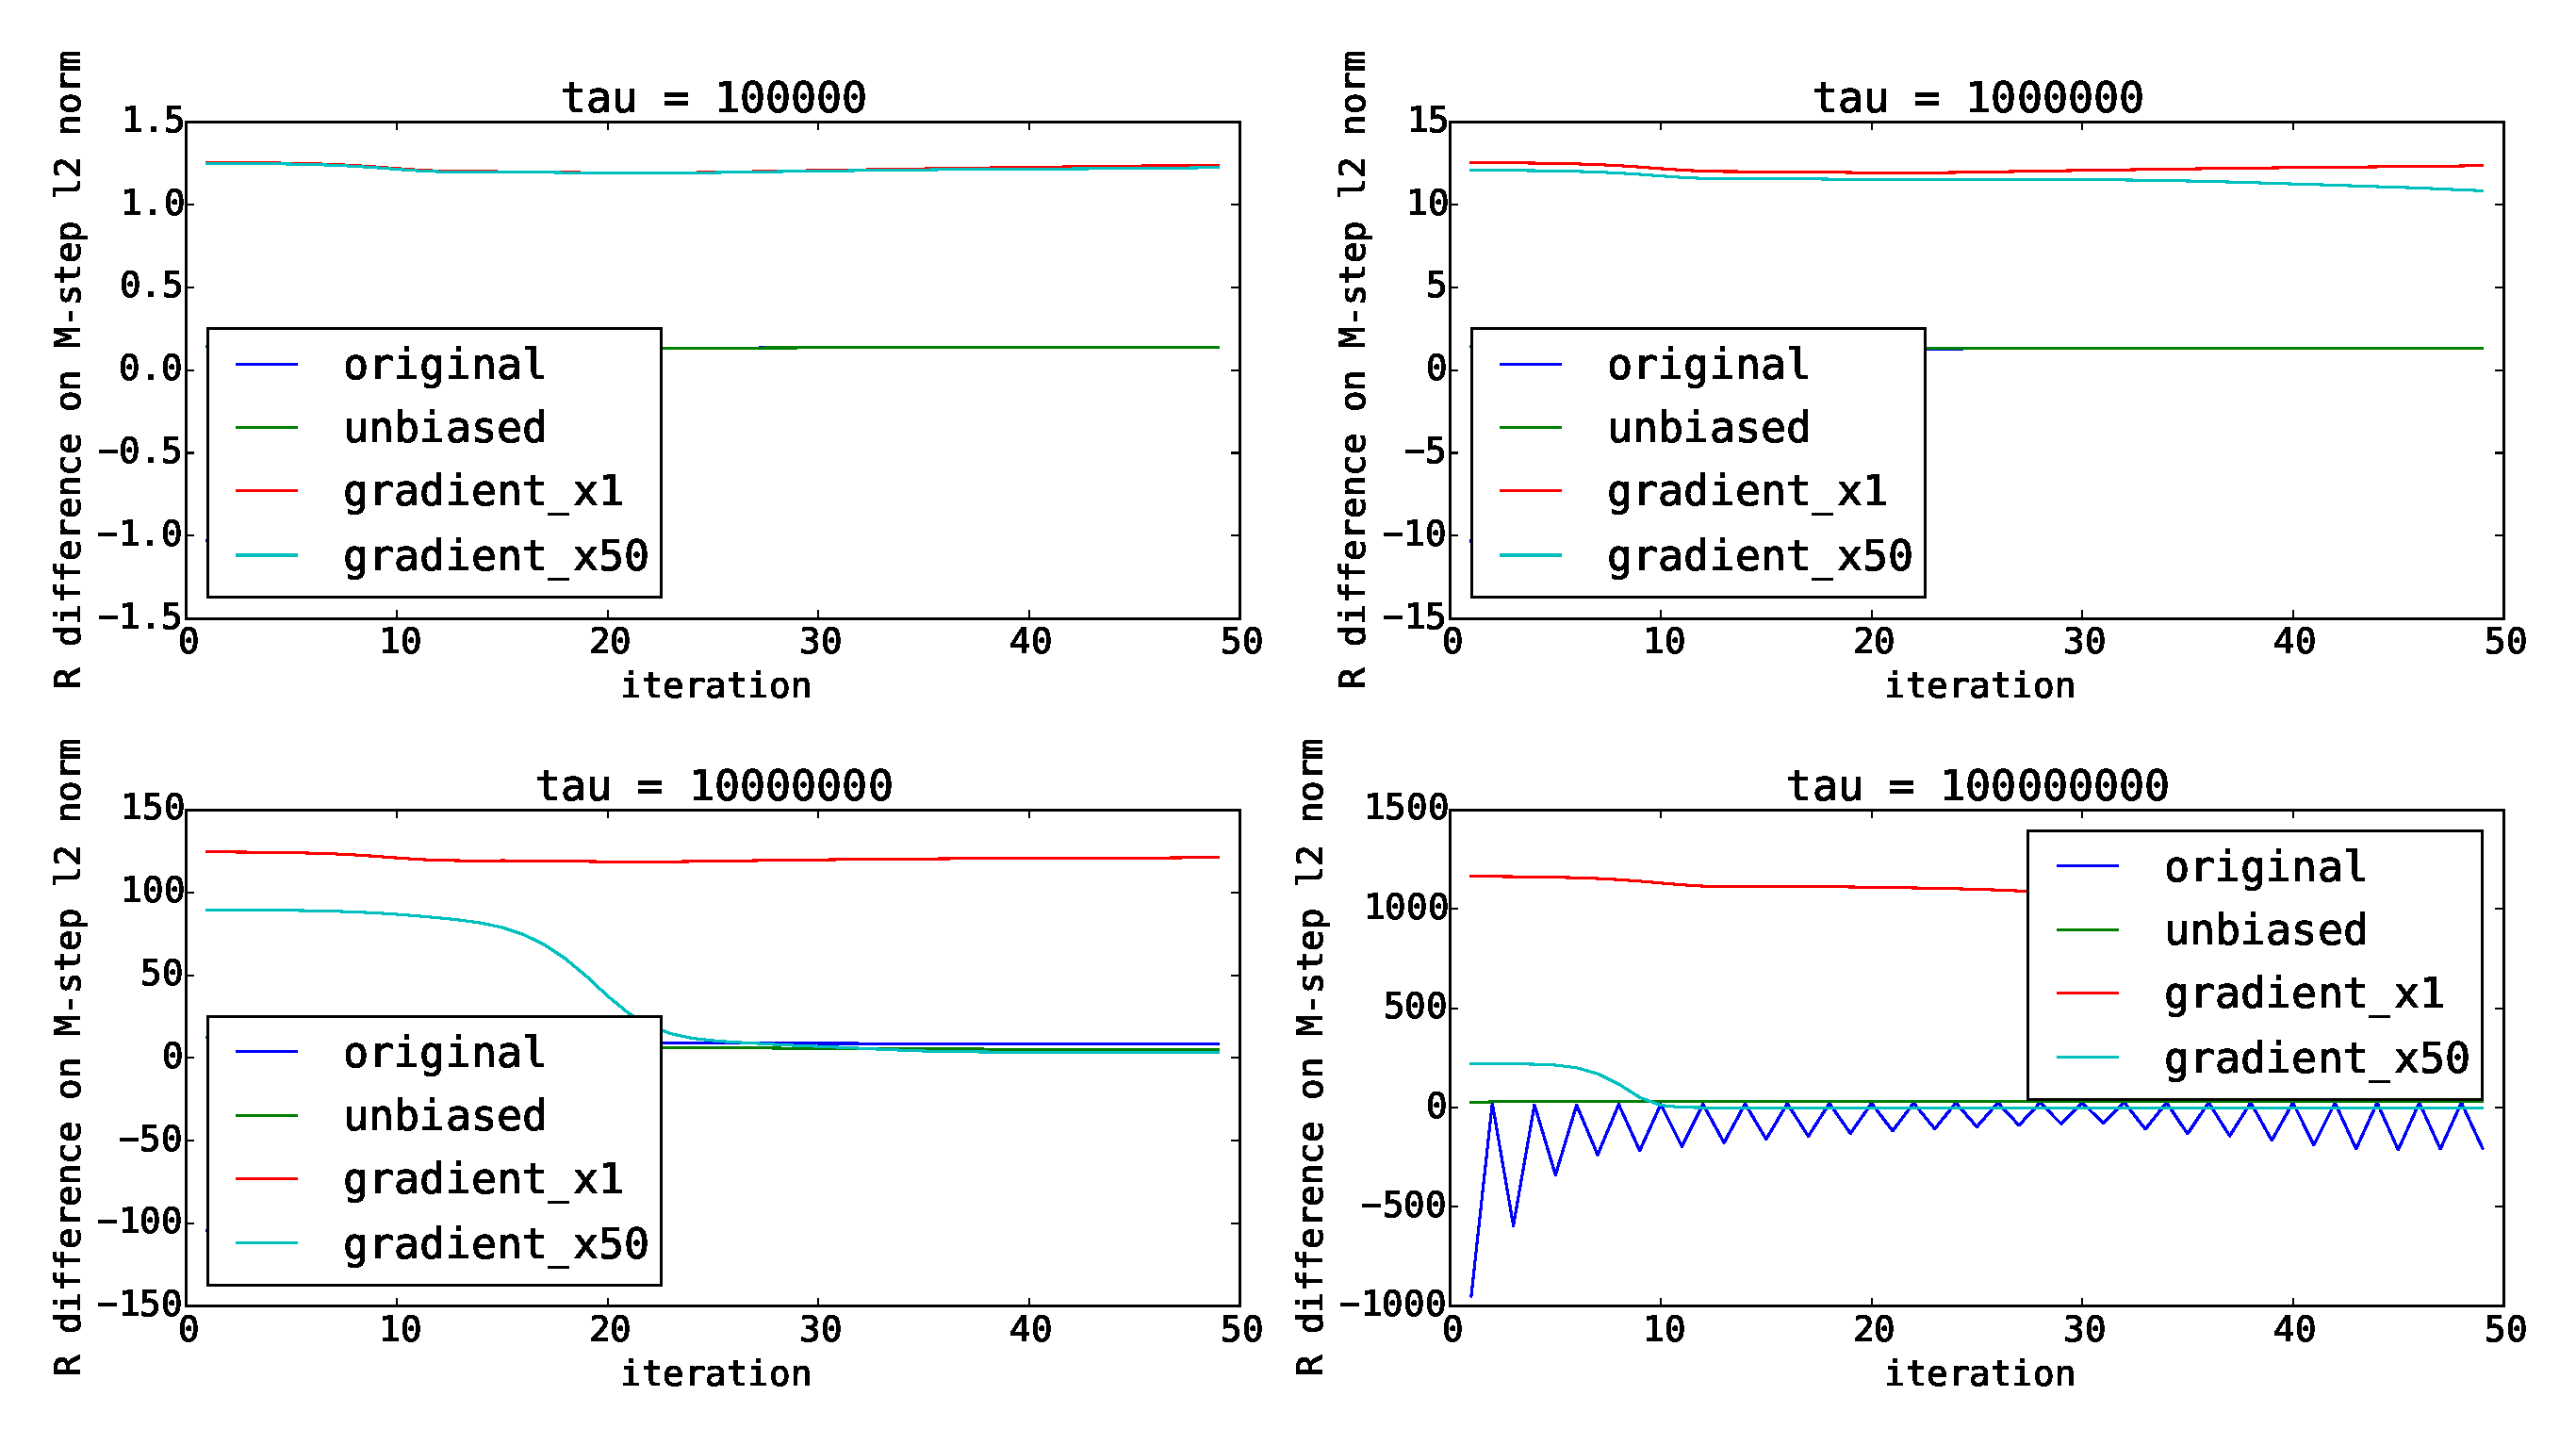
\includegraphics[width=1.0\linewidth]{presentation_pictures/topics_10_RMstepDiffPerL2}
\end{figure}
	\end{frame}
	
	\begin{frame}
\begin{figure}
	\centering
	\caption{Логарифм минимального ненулевого значения матрицы $\Phi$. $|T| = 10$.}    
	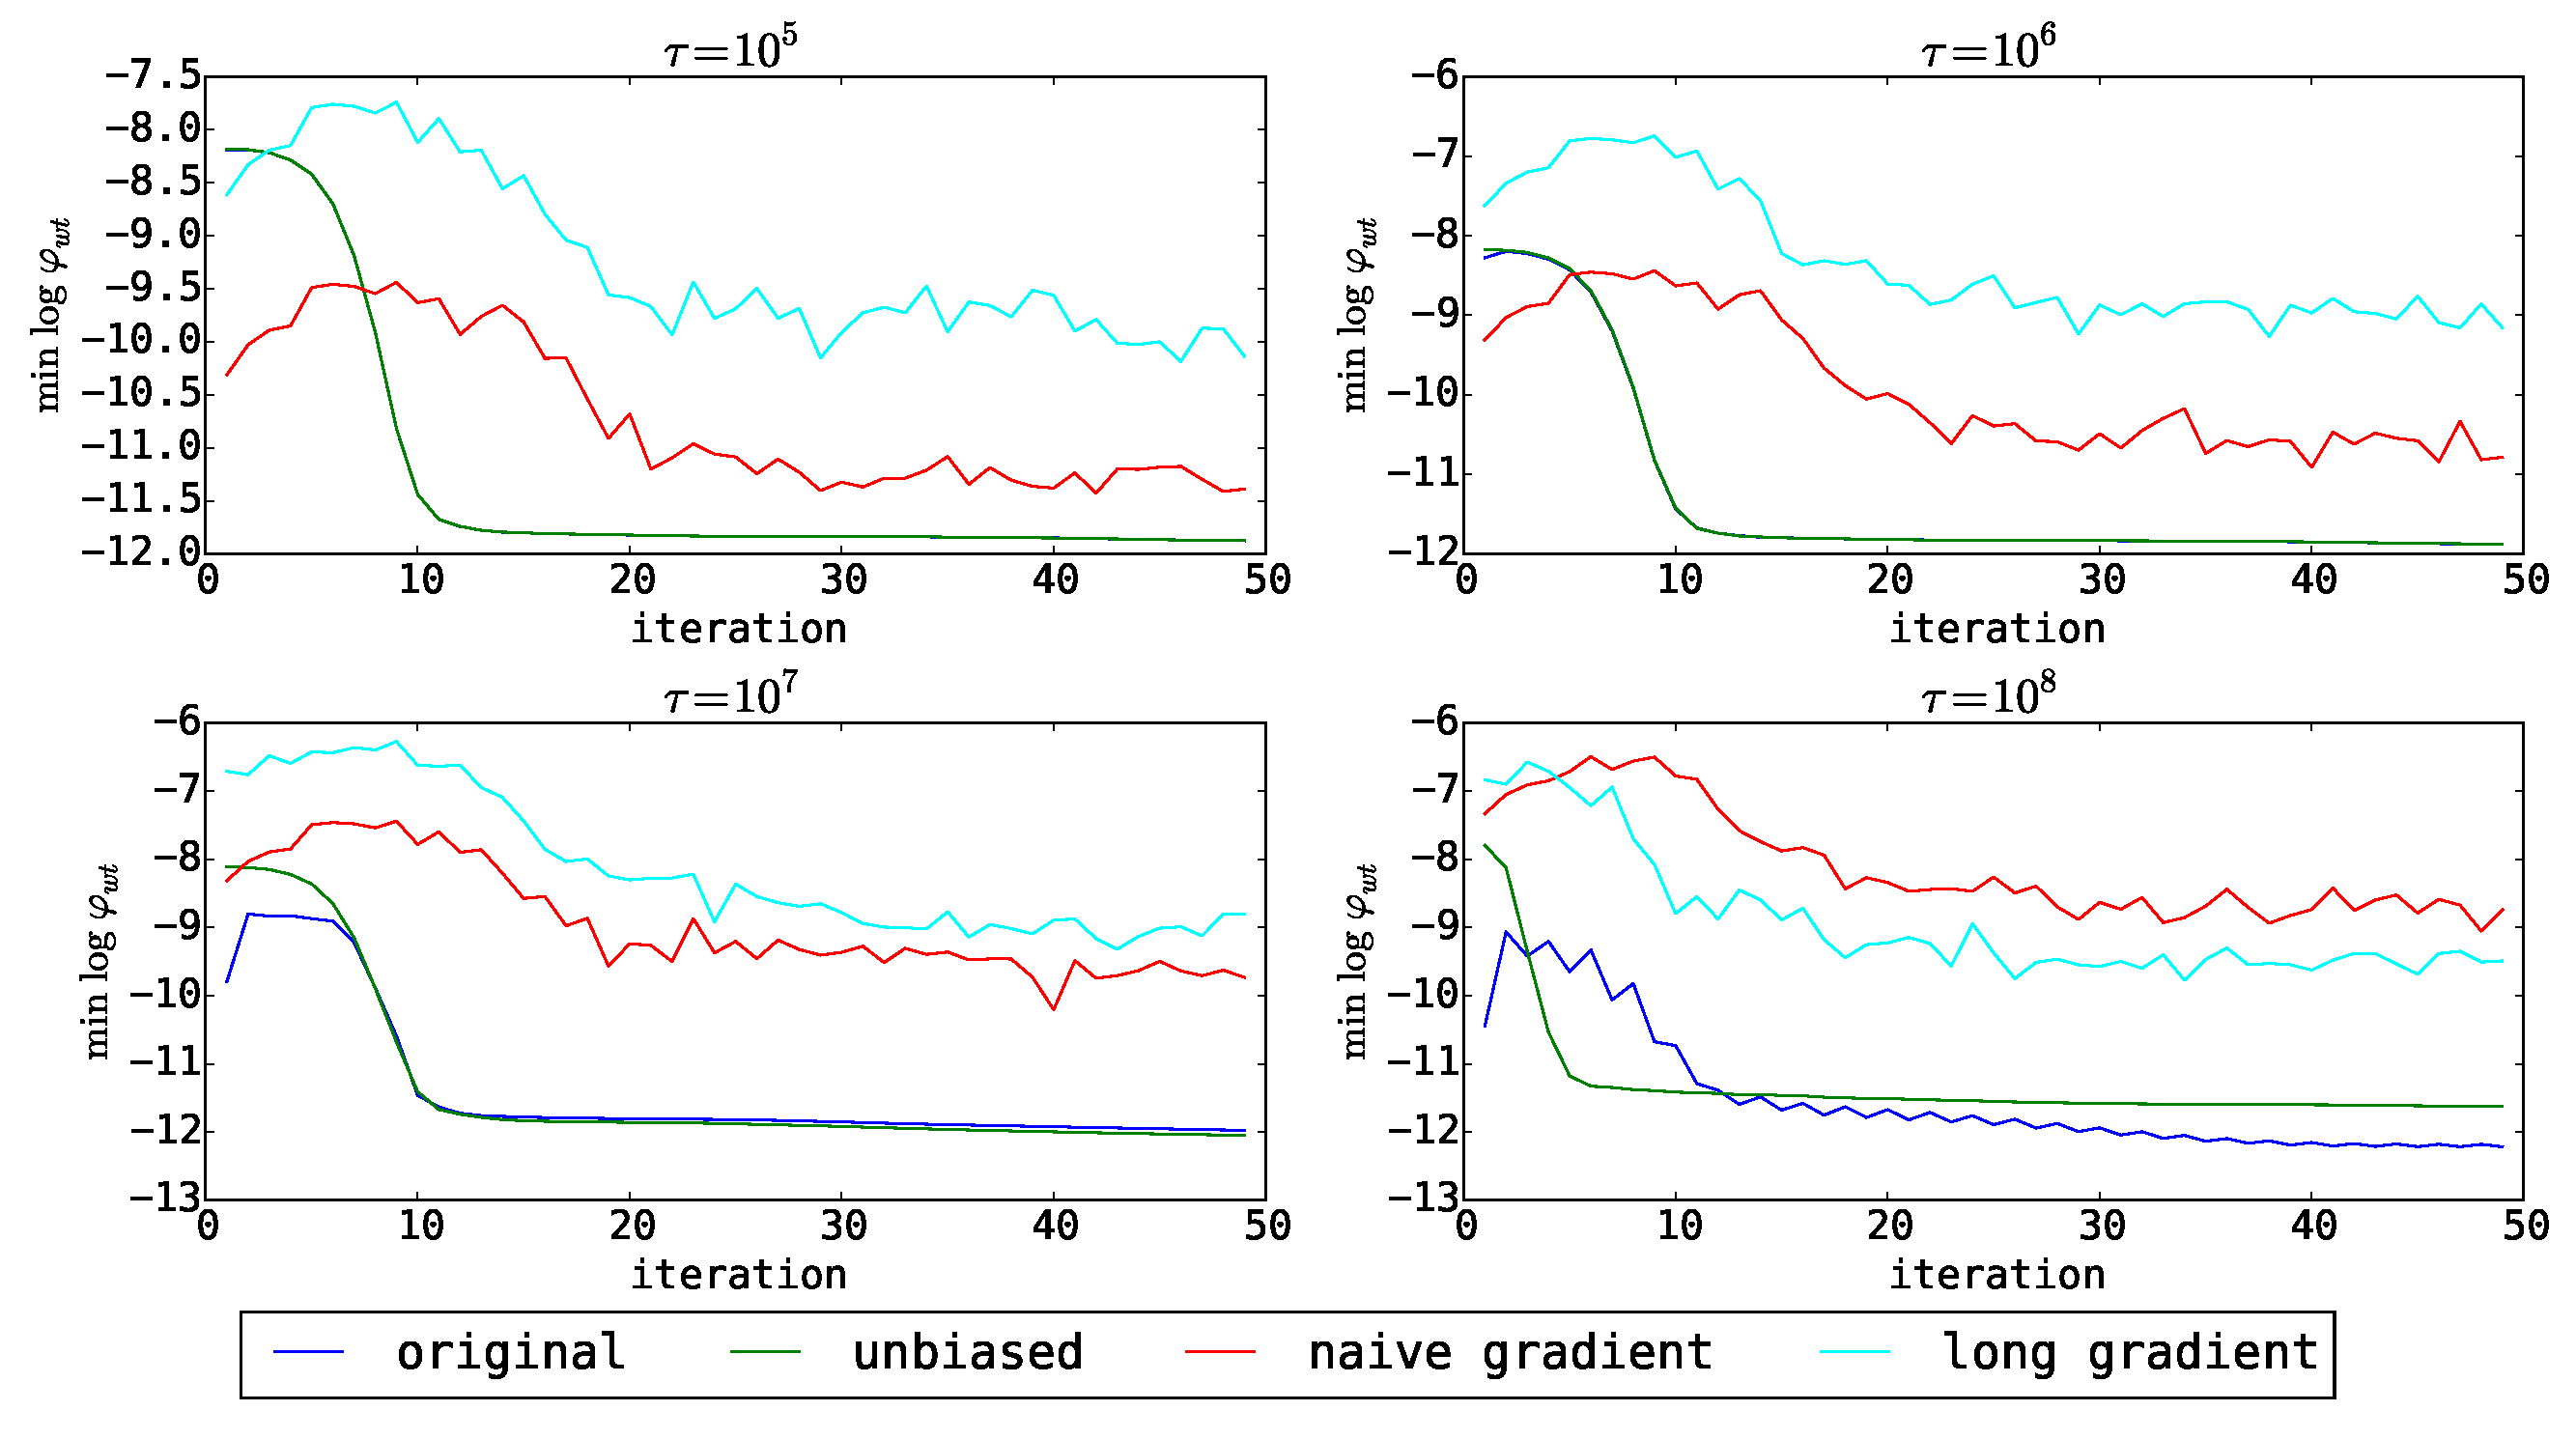
\includegraphics[width=1.0\linewidth]{presentation_pictures/topics_10_minPhi_values}
\end{figure}
	\end{frame}
	
\begin{frame}{Итоги экспериментов}
\begin{enumerate}
\item Предположения об отделимости и невырожденности распределений выполняются на практике.
\item С точки зрения оптимизации $L + \tau R$ все рассмотренные формулы отличаются незначительно. Основное достоинтсво предложенных модификаций в этом плане --- это теоретические гарантии.
\item Есть эффект скачков значений функционалов на первых итерациях для стандартной формулы, вызванный выбором точки в которой считаются $r_{wt}$ и $r_{td}$.
\item Для градиентных поправок необходимо дополнительное исследование, чтобы понять как подбирать константу перед градиентом.
\end{enumerate}
\end{frame}

	\begin{frame}{Краткое резюме}
 \begin{enumerate}
\item  Получены условия сходимости ЕМ-алгоритма для максимизации аддитивно регуляризованного правдоподобия в задачах тематического моделирования.
\item Получены условия сходимости, показано, что они не являются слишком жёсткими. 
\item Предложены модификации ЕМ-алгоритма, улучшающие сходимость регуляризованного ЕМ-алгоритма.
\end{enumerate}
	\end{frame}

\end{document}
